% document type
\documentclass[12pt]{article}

% packages
\usepackage{amsmath} % for mathematical symbols and environments
\usepackage{amsfonts} % for additional math fonts
\usepackage{amssymb} % for additional math symbols
\usepackage{hyperref} % for hyperlinks
\usepackage{geometry}
\usepackage{bookmark}

\usepackage{tikz} % for graphics
\usetikzlibrary{arrows,shapes}

% title and author
\title{Numeric to Symbolic to Parametric space of solutions of Polynomial Systems of Equations}
\author{Ilay Menahem, Michael Shalyt, Ido Kaminer}

% article text
\begin{document}

\maketitle

% abstract
\begin{abstract}
    There is a problem shared among many fields of science of solving polynomial systems of equations.
    The required solution is often a space of solutions, rather than a single solution.
    Applications include QFT, robotics, cryptography, optimization, chemistry, electrical engineering, and more. [we need other examples... best is to have concrete examples from history. If not then maybe say generally that in many areas of science and engineering a parametric solution can surprise us and help where our creativity is limited].

    This paper presents a scalable pipeline for finding a space of solutions (of full dimension) to polynomial systems of equations.
    We start from numerical solutions, transitioning to symbolic solutions, and finally parametrize the solution space via structured exploration.
    We then also discuss other complementary methods and discuss what open questions still remain.
    We demonstrate these methods on concrete examples from the field of QFT. 
\end{abstract}

\section*{Introduction}
Solving polynomial systems of equations is a fundamental problem in mathematics and computer science, with applications in fields such as robotics, cryptography, optimization, QFT, chemistry, electrical engineering, economics and more.
In QFT, polynomial systems arise in the context of generilizing and unifying theories (e.g. quantum gravity). 
In chemistry, for example, polynomial systems appear in the study and design of reaction chains.
In robotics, for example, polynomial systems are used to model kinematics and motion planning.

In most of these use cases, the required solution is often a space of solutions, rather than a single solution.
Specifically, in QFT the proposed theory must follow gauge invariance, which leads to a space of solutions, and of these solutions one may want to find the one represents the simplest theory.
In chemistry, reaction chains often have multiple valid pathways, leading to a solution space.
In robotics, the solution space may represent all possible configurations of a robotic arm that satisfy certain constraints. one would want to work with the entire solution space to find optimal paths and configurations.
This type of problem is universal across many fields of science and engineering. It calls for a comprehensive approach that can efficiently find and represent the solution space of polynomial systems.

% classic methods for solving polynomial systems of equations
Classic methods for solving polynomial systems of equations include Groebner bases [], resultants [], and homotopy continuation []. However, these methods can be computationally expensive and may not scale well with the size of the system. Other approaches, such as gradient [], and SMT solvers [] are focused on finding specific solutions rather than exploring the entire solution space.

% overview of the proposed pipeline
In this paper, classify/group/review/discuss specially made approaches for finding the general ... in efficient ways relevant for.
We also demonstrate the methods on concrete examples from QFT.
Among those methods, we propose a pipeline that leverages numerical methods to find initial solutions, then refines these solutions into symbolic forms, and finally explores a space of solutions. This approach aims to combine the efficiency of numerical methods, and some insights we may have at how the symbolic solutions may look like, to provide a comprehensive understanding of a solution space of polynomial systems.
We also present and analyze a complementary examples from QFT, showcasing the effectiveness of our approach in practical scenarios.
We finally outline the open questions and future directions [more concrete] in this field.


\section*{Mathematical Background}
Let $\mathbb{K}[\mathbf{x}]$ denote the polynomial ring in variables $\mathbf{x} = (x_1, \ldots, x_n)$ over a field $\mathbb{K}$, typically $\mathbb{R}$ or $\mathbb{C}$. A polynomial system is defined by a map $F: \mathbb{K}^n \to \mathbb{K}^m$ with components $f_1, \ldots, f_m \in \mathbb{K}[\mathbf{x}]$. The locus of simultaneous solutions constitutes the \textit{affine variety} $V(F) = \{ \mathbf{a} \in \mathbb{K}^n \mid F(\mathbf{a}) = \mathbf{0} \}$.

\noindent given a smooth system of equations $F\in C_\infty$ (possibly polynomial) with a solution point $p$, one can find the dimension of the solution space around that point using its Jacobian at that point $J_F(p)$. the following theorem formalizes this idea.

\noindent\textbf{Theorem:} 
Let $F: U \subseteq \mathbb{K}^m \to \mathbb{K}^n$ be a smooth map defined on an open set $U$, with components $F = (f_1, \ldots, f_n)$. Let $p \in U$ be a point such that $F(p) = \mathbf{0}$. If the Jacobian matrix $J_F(p)$ has rank $r$, then there exists a neighborhood $V$ of $p$ such that the solution set $F^{-1}(\mathbf{0}) \cap V$ is a smooth manifold of dimension $m - r$.

\noindent\textbf{Proof:}
--- need to fill in ---


\section*{What is a solution?}
there are a few ways to interpret the meaning of the solution to a system of equations.
\begin{list}{-}{}
    \item \textbf{numerical solutions:} specific numerical values for the variables that satisfy all equations in the system (with very high precision).
    \item \textbf{symbolic solutions:} symbolic expressions of constants that satisfy all equations in the system.
    \item \textbf{lowest norm solution:} a solution numerical or symbolic, that minimizes some norm. for example, $L_0$ norm minimization leads to the sparsest solution, while $L_2$ norm minimization leads to the solution with the smallest Euclidean length.
    \item \textbf{parametric expression of a variety:} a set of symbolic or numerical approximated expressions, that provide a parametric representation of the set of all possible solutions to the system. the set of system solutions is also known as the variety. there are various ways to represent the variety parametrically, such as rational, polynomial, or trigonometric parametrizations. yet there are some varieties that cannot be parametrized such as elliptic curves.
    \item \textbf{point cloud sampling of the variety:} a large set of numerical or symbolic solutions that sample the variety, which can be used to understand its structure and properties.
\end{list}


\section*{Moving between types of solutions}
one can note that it is fairly straightforward to find certain types of solutions such as numerical solutions via Newton-Raphson, but sometimes it is more desirable to have symbolic solutions or parametric expressions of the variety. in the diagram below, we illustrate the different types of solutions and the methods we will use to move between them.

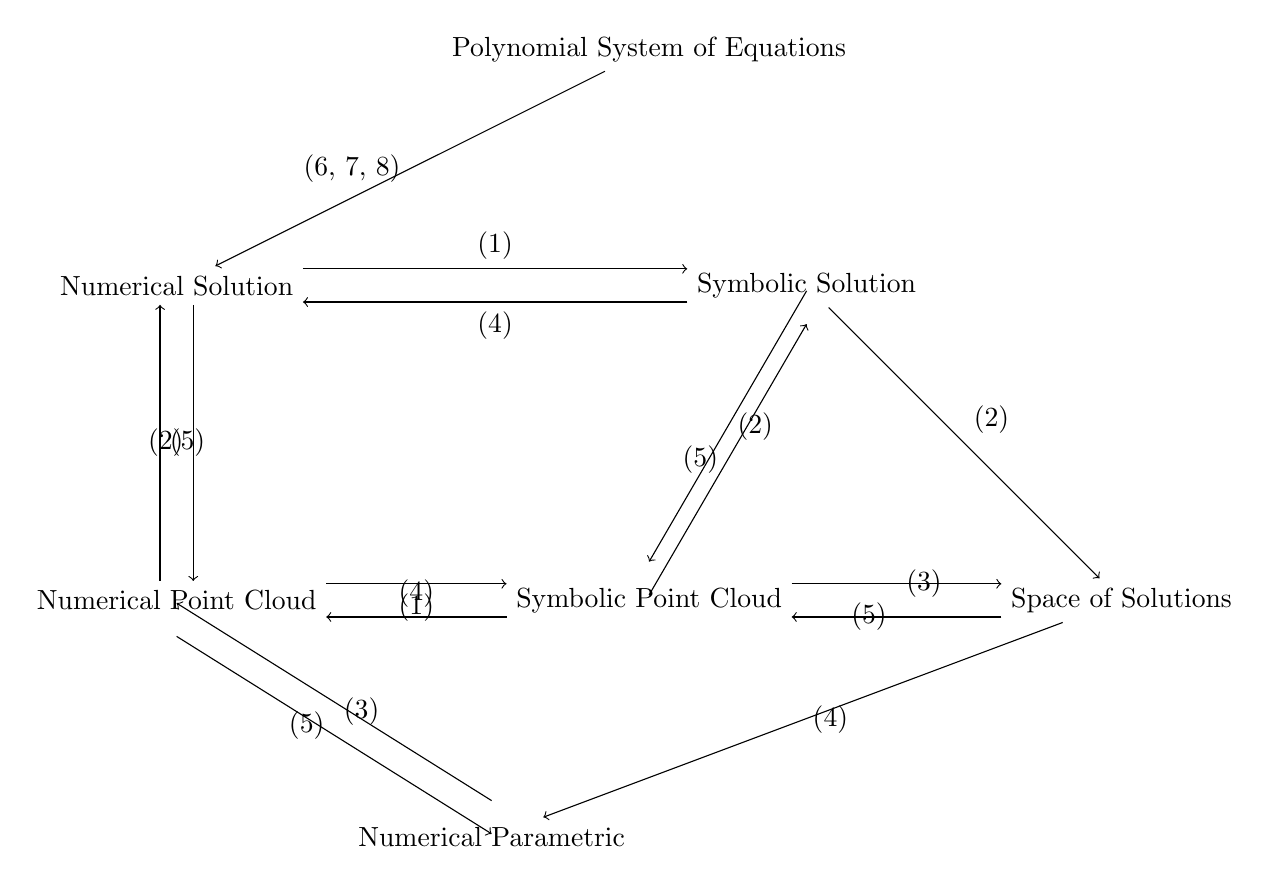
\begin{tikzpicture}[node distance=2cm]
% spread out layout
    \node (start) at (6,0) {Polynomial System of Equations};
    \node (numerical) at (0,-3) {Numerical Solution};
    \node (symbolic) at (8,-3) {Symbolic Solution};
    \node (num_cloud) at (0,-7) {Numerical Point Cloud};
    \node (sym_cloud) at (6,-7) {Symbolic Point Cloud};
    \node (parametric) at (12,-7) {Space of Solutions};
    \node (num_parametric) at (4,-10) {Numerical Parametric};

    % Straight arrows (no bends)
    \draw[->] (start) -- (numerical) node[midway, left] {(6, 7, 8)};
    \draw[->] ([yshift=6pt]numerical.east) -- ([yshift=6pt]symbolic.west) node[midway, above] {(1)};
    \draw[->] ([yshift=-6pt]symbolic.west) -- ([yshift=-6pt]numerical.east) node[midway, below] {(4)};
    \draw[->] ([xshift=6pt]numerical.south) -- ([xshift=6pt]num_cloud.north) node[midway, left] {(2)};
    \draw[->] ([yshift=6pt]symbolic.south) -- ([yshift=6pt]sym_cloud.north) node[midway, right] {(2)};
    \draw[->] ([xshift=-6pt]num_cloud.north) -- ([xshift=-6pt]numerical.south) node[midway, right] {(5)};
    \draw[->] ([yshift=-6pt]sym_cloud.north) -- ([yshift=-6pt]symbolic.south) node[midway, left] {(5)};
    \draw[->] ([yshift=6pt]num_cloud.east) -- ([yshift=6pt]sym_cloud.west) node[midway, below] {(1)};
    \draw[->] ([yshift=-6pt]sym_cloud.west) -- ([yshift=-6pt]num_cloud.east) node[midway, above] {(4)};
    \draw[->] ([yshift=6pt]sym_cloud.east) -- ([yshift=6pt]parametric.west) node[midway, right] {(3)};
    \draw[->] ([yshift=-6pt]parametric.west) -- ([yshift=-6pt]sym_cloud.east) node[midway, left] {(5)};
    \draw[->] (symbolic) -- (parametric) node[midway, above right] {(2)};
    \draw[->] (parametric) -- (num_parametric) node[midway, right] {(4)};
    \draw[->] ([yshift=6pt]num_parametric.north) -- ([yshift=6pt]num_cloud.south) node[midway, below left] {(5)};
    \draw[->] ([yshift=-6pt]num_cloud.south) -- ([yshift=-6pt]num_parametric.north) node[midway, above right] {(3)};
\end{tikzpicture}

\begin{enumerate}
    \item \textbf{PSLQ and numerical fitting:} in this method, we use the PSLQ algorithm to find integer relations in the numerical solutions, replace numerical results with symbolic expressions, refit the solution and repeat until we have replaced all numerical values with symbolic expressions.
    \item \textbf{Going penpendicular to Jacobian null space:} given a solution to the polynomial system of equations, and if we will go in a direction that is perpendicular to the Jacobian null space at that point, we will remain in the solution space of the system. by taking small steps in such directions, we can sample more solutions to the system.
    \item \textbf{Symbolic regression:} given a point cloud of solutions, we can use symbolic regression to find parametric expressions that fit the point cloud.
    \item \textbf{Evaluating symbolic expressions:} given symbolic expressions, we can evaluate them to get numerical solutions.
    \item \textbf{Sampling points:} given numerical or symbolic parametric expressions of the variety, we can sample points from them to get point clouds of solutions.
    \item \textbf{SMT solvers:} SMT solvers can sometimes be used to find symbolic or numerical solutions to systems of equations.
    \item \textbf{Newton-Raphson:} given a system of equations, we can use the Newton-Raphson method to find numerical solutions to the system.
    \item \textbf{Homotopy continuation:} Homotopy continuation methods take a system of equations with known solutions and continuously deform it into the target system, tracking the solutions throughout the deformation process to find solutions to the original system.
\end{enumerate}


\section*{Linear elimination}

even in the case of very large non linear polynomial systems of equations, it is possible to eliminate variables in a linear fashion, which can significantly reduce the size of the system and the number of variables.
\\\textbf{input:} polynomial system of equations $P = \{p_1, p_2, \ldots, p_k\} \subseteq \mathbb{K}[x_1, x_2, \ldots, x_m]$.
\\\textbf{output:} a polynomial system of equations $Q = \{q_1, q_2, \ldots, q_k\}$, which is equivalent to $P$, and each $q_i$ is a not linear in any variable $x_j$ for $j \in \{1, 2, \ldots, m\}$.
\\\textbf{algorithm:}
\begin{enumerate}
    \item Let $L = \{(x_j, p_i) | p_i \text{ is linear in } x_j\}$ be the list of all variables and polynomials that are linear in those variables.
    \item Let $V = \{x_1, x_2, \ldots, x_m\}$ be the set of all variables.
    \item Let $Q = P$ be the output polynomial system of equations.
    \item While $L$ is not empty:
    \begin{enumerate}
        \item Select a variable-polynomial pair $(x_j, p_i)$ from $L$.
        \item Remove $(x_j, p_i)$ from $L$, $x_j$ from $V$, and $p_i$ from $Q$.
        \item Solve $p_i$ for $x_j$: $x_j = f(\hat{x})$.
        \item For each polynomial $p_k$ in $Q$ substitute $x_j$ with $f(\hat{x})$.
        \item Update $L$ to reflect the changes in $Q$.
    \end{enumerate}
\end{enumerate}

in the example below, we demonstrate that for systems of low degree polynomials, this method can significantly reduce the number of variables and equations in the system, without increasing the degree of any polynomial in the system.

--- add the example ---

\section*{Numerical solutions via Newton-Raphson}
to apply the Newton-Raphson method to an underdetermined system of equations we can use the following update step\cite{BenIsrael1966ANM}: \[x_{n+1} = x_n - J^+(x_n) F(x_n)\] where $J^+$ is the Moore-Penrose pseudoinverse of the Jacobian matrix $J$ of $F$ at point $x_n$.

% minimizing the $L_1$ norm to improve solution sparsity and stability of Newton-Raphson
it is well known that minimizing the $L_1$ norm of the solution can lead to sparser solutions [], and can also improve the stability of the Newton-Raphson method []. % write more about methods for sparsity and stability

\section*{Symbolic solutions via iterations of PSLQ and Newton-Raphson}
if we have a numerical solution in neighborhood of solutions of dimension $k$, one of the simplest ways to convert it to a parametric solution would to covert some of the entries of the numerical solution to symbolic fractions of close values. the following theorem formalizes this idea.
\\\textbf{theorem:} let there be a $k$ dimensional manifold (can be a solution space of a polynomial system of equations) embedded in an $n$ dimensional space. there is a point in the manifold, such that $k$ of the $n$ coordinates are rational.
\\\textbf{proof:} 


\section*{exploration of space of solutions}
here we present a theorem regarding given one solution how can we derive a neighborhood of solutions to any system of equations via the Jacobian null space at that point.
\\\textbf{theorem:} let $F = \{f_1, f_2, \ldots, f_n\}$ be a system of smooth functions in variables $x = (x_1, x_2, \ldots, x_m)$. let $J$ be the Jacobian matrix of $F$ with respect to $x$, $x_0$ be a point such that $F(x_0) = 0$, and $v \in N(J(x_0))$ be a vector in the null space of $J$ at point $x_0$. 
then $\frac{d}{dt}F(x_0 + tv)|_{t=0} = 0$.
\\\textbf{proof:} By the multivariable chain rule, the derivative of the composition $F(x_0 + tv)$ with respect to $t$ is given by:
\[\frac{d}{dt}F(x_0 + tv) = J(x_0 + tv) \cdot \frac{d}{dt}(x_0 + tv) = J(x_0 + tv) \cdot v\] 
Evaluating this expression at $t=0$: \[\frac{d}{dt}F(x_0 + tv)\bigg|_{t=0} = J(x_0) \cdot v\]
Since $v$ is in the null space of $J(x_0)$, we have $J(x_0)v = 0$. Thus: \[ \frac{d}{dt}F(x_0 + tv)\bigg|_{t=0} = 0 \]

a use of this theorem to extract a parametric solution from a symbolic one is in the appendix.

\subsection*{Numerical exploration of space of solutions}

\subsection*{Symbolic exploration of space of solutions}

\section*{Finding the whole space of solutions}
After parametrizing a set of solutions, one may want to ensure that the entire solution space has been found. For that one can Rabinowitsch Trick to add an additional constraint to the system of equations that excludes the already found solutions, and then attempt to find new solutions to the modified system. If no new solutions are found, it can suggest that the entire solution space has been explored.

% A simple example of applying this method is provided in the appendix.

\section*{Appendix}
\subsection*{Derivation of neighborhood of solutions via Jacobian null space}
system of polynomial equations:
\begin{align*}
f_1 &= x^2 + y^2 + z^2 - 1 = 0 \\
f_2 &= x + y + z - 1 = 0
\end{align*}
Let us choose a solution $x_0 = (1, 0, 0)$. We can verify that $f_1(1,0,0) = 1^2 + 0 + 0 - 1 = 0$ and $f_2(1,0,0) = 1 + 0 + 0 - 1 = 0$.

The Jacobian matrix $J$ is given by:
\[
J = \begin{pmatrix}
\frac{\partial f_1}{\partial x} & \frac{\partial f_1}{\partial y} & \frac{\partial f_1}{\partial z} \\
\frac{\partial f_2}{\partial x} & \frac{\partial f_2}{\partial y} & \frac{\partial f_2}{\partial z}
\end{pmatrix} = \begin{pmatrix}
2x & 2y & 2z \\
1 & 1 & 1
\end{pmatrix}
\]
Evaluating $J$ at $x_0 = (1, 0, 0)$:
\[
J(x_0) = \begin{pmatrix}
2 & 0 & 0 \\
1 & 1 & 1
\end{pmatrix}
\]
To find the null space, we solve $J(x_0)v = 0$ for $v = (v_x, v_y, v_z)^T$:
\[
\begin{pmatrix}
2 & 0 & 0 \\
1 & 1 & 1
\end{pmatrix} \begin{pmatrix}
v_x \\ v_y \\ v_z
\end{pmatrix} = \begin{pmatrix}
0 \\ 0
\end{pmatrix}
\]
From the first row, $2v_x = 0 \implies v_x = 0$.
From the second row, $v_x + v_y + v_z = 0 \implies 0 + v_y + v_z = 0 \implies v_y = -v_z$.
Let $v_z = 1$, then $v_y = -1$. Thus, a vector in the null space is $v = (0, -1, 1)^T$.

Moving from $x_0$ in the direction of $v$ keeps the system approximately solved to the first order. moving the direction of $v$ can be done numerically by choosing a small $t$, evaluating $x(t) = x_0 + tv$, and doing a Newton-Raphson step to refine the solution.

To perform the symbolic walk, we calculate the null space of $J$ symbolically. The null space direction $v(x,y,z)$ must satisfy $J v = 0$, which means $v$ is orthogonal to the gradients of $f_1$ and $f_2$. This direction is given by the cross product of the gradients (ignoring the scalar factor 2 from $\nabla f_1$):
\[
v(x,y,z) = \frac{1}{2}\nabla f_1 \times \nabla f_2 = \begin{pmatrix} x \\ y \\ z \end{pmatrix} \times \begin{pmatrix} 1 \\ 1 \\ 1 \end{pmatrix} = \begin{pmatrix} y-z \\ z-x \\ x-y \end{pmatrix}
\]
This yields the system of differential equations:
\begin{align*}
\dot{x} &= y - z \\
\dot{y} &= z - x \\
\dot{z} &= x - y
\end{align*}
Solving this system with initial condition $x(0) = (1, 0, 0)$ yields the parametric solution for the variety.

Adding the three equations gives $\dot{x} + \dot{y} + \dot{z} = 0$, implying $x+y+z = C_1$. From the initial condition, $1+0+0=1$, so $x+y+z=1$.
Differentiating $\dot{x}$ gives $\ddot{x} = \dot{y} - \dot{z} = (z-x) - (x-y) = z+y-2x$. Substituting $y+z = 1-x$, we get $\ddot{x} = (1-x) - 2x = 1 - 3x$.
This is a linear ODE $\ddot{x} + 3x = 1$. The homogeneous solution is $A\cos(\sqrt{3}t) + B\sin(\sqrt{3}t)$, and the particular solution is $x_p = 1/3$.
So $x(t) = A\cos(\sqrt{3}t) + B\sin(\sqrt{3}t) + 1/3$.
Using $x(0)=1$, we get $A + 1/3 = 1 \implies A = 2/3$.
Using $\dot{x}(0) = y(0)-z(0) = 0$, we get $\sqrt{3}B = 0 \implies B=0$.
Thus $x(t) = \frac{2}{3}\cos(\sqrt{3}t) + \frac{1}{3}$.
By symmetry and the cyclic nature of the equations, the solutions for $y$ and $z$ are phase-shifted or can be derived similarly.
Since $\dot{x} = y-z$ and $y+z = 1-x$, we have a system for $y,z$:
$y-z = -\frac{2}{\sqrt{3}}\sin(\sqrt{3}t)$ and $y+z = 1 - (\frac{2}{3}\cos(\sqrt{3}t) + \frac{1}{3}) = \frac{2}{3} - \frac{2}{3}\cos(\sqrt{3}t)$.
Adding these: $2y = \frac{2}{3} - \frac{2}{3}\cos(\sqrt{3}t) - \frac{2}{\sqrt{3}}\sin(\sqrt{3}t) \implies y(t) = \frac{1}{3} - \frac{1}{3}\cos(\sqrt{3}t) - \frac{1}{\sqrt{3}}\sin(\sqrt{3}t)$.
Subtracting: $2z = \frac{2}{3} - \frac{2}{3}\cos(\sqrt{3}t) + \frac{2}{\sqrt{3}}\sin(\sqrt{3}t) \implies z(t) = \frac{1}{3} - \frac{1}{3}\cos(\sqrt{3}t) + \frac{1}{\sqrt{3}}\sin(\sqrt{3}t)$.

The parametric solution is:
\begin{align*}
x(t) &= \frac{1}{3} + \frac{2}{3}\cos(\sqrt{3}t) \\
y(t) &= \frac{1}{3} - \frac{1}{3}\cos(\sqrt{3}t) - \frac{1}{\sqrt{3}}\sin(\sqrt{3}t) \\
z(t) &= \frac{1}{3} - \frac{1}{3}\cos(\sqrt{3}t) + \frac{1}{\sqrt{3}}\sin(\sqrt{3}t)
\end{align*}

\bibliographystyle{plain}
\bibliography{references}

\end{document}